\titre{Principe :} Calculer le coût moyen de chaque opération dans le pire cas de séquence d'opérations. \\

\titre{3 techniques standard :}
\begin{itemize}
	\item Méthode par agrégat
	\item Méthode comptable
	\item Méthode du potentiel
\end{itemize}

\titre{Méthode par agrégat :} On montre que pour toute suite d'opérations, le temps total est $T(n)$ dans le pire cas et le cout amorti (= cout moyen) de chaque opération est $\frac{T(n)}{n}$. \\

\titre{Exemple : La pile } \\
On a 3 opérations sur les piles :
\begin{itemize}
	\item Empiler(S,x) $\theta(1)$
	\item Depiler(S) $\theta(1)$
	\item Multidepiler{S,k} $\theta(min(k,s))$ ($s=$Card$S$)
\end{itemize}
L'utilisateur faire une série de $n$ opérations parmi ces 3 là.
\begin{itemize}
	\item $n$ fois empiler,depiler $\theta(n)$
	\item $n$ Multidepiler Cout borné par les $k$ choisis et le nombre d'éléments de la pile
	\item $\frac{n}{2}$ empiler et $\frac{n}{2}$ multidépiler Donc $\frac{n}{2}\theta(n) = O(n^2)$
\end{itemize}
En réalité, on empile et dépile $n$ fois quoi qu'il arrive donc la complexité en pire cas est $\theta(n)$\\
Cout amorti de chaque opération = Cout total / $n$ = $\theta(1)$

\titre{Exemple : Le compteur de bits}\\
On a un tableau $A[0..k-1]$ de bits. Donc $A$ représente un entier $x=\displaystyle{\sum_{i=0}^kA[i]2^i}$ qu'on appelle le compteur.\\
On a l'opération incrémenter qui ajoute 1 à $x$ \\
\\
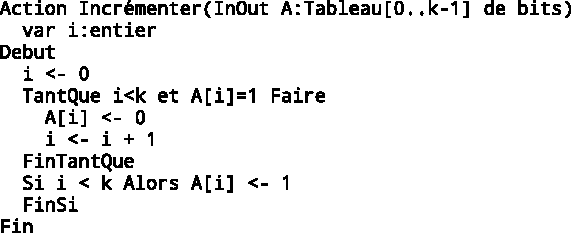
\includegraphics{Images/fig1.pdf}
\\
On compte le nombre de fois que chaque bit est modifié \\
Cout total = $n\displaystyle{\sum_{i=0}^{k'}}(\frac{1}{2})^{k'}$ avec $k'=\log_2 n$ donc Cout total $\leq 2n$ \\
Le cout amorti est donc $\theta(1)$

